\chapter{Developer Tooling}
\label{chap-dev-tooling}

\renewcommand{\headrulewidth}{0.3pt}
\fancyhead[LE]{\thepage} \fancyhead[RE]{\nouppercase{\textbf{\leftmark}}}
\fancyhead[RO]{\thepage} \fancyhead[LO]{\nouppercase{\textbf{\rightmark}}}
\fancyfoot[L,C,R]{}

\setlength{\parindent}{0.35cm}

\minitoc
\newpage
% ================================================================

This chapter covers the \textbf{optional tools} that make day-to-day development easier: the debugging utilities (plugin reloading, error inspection, and a full VS-Code debugger attached to QGIS), and \script{Qt Designer} for authoring dialog boxes.

\section{Debugging Tools}
\subsection{The \script{Plugin Reloader} plugin}

This utility allows reloading a plugin after a code modification. Thus it is not necessary to reload QGIS after each code change.

The plugin can be installed from the \script{QGIS} extension manager.

\begin{figure}[H]
    \centering
    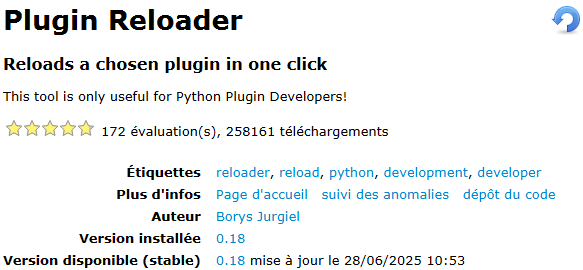
\includegraphics[width=0.75\linewidth]{9_developer_tooling/fig/plugin_reloader.png}
    \caption{Description sheet for \script{Plugin Reloader}}
    \label{fig_plugin_reloader}
\end{figure}

\subsection{The QGIS plugin \script{First Aid}}

The \script{First Aid} plugin allows investigating errors occurring during plugin execution.


\newpage
\subsection{VS-Code}
The \script{debugvs} plugin allows connecting a \script{VS-Code} debugging instance to the plugin execution from QGIS. This debugging configuration allows using all VS Code features during debugging (breakpoints, watch, call stack...). Setting up this debugging configuration is done as follows:
\begin{enumerate}
    \item install \script{debugpy} with the command \script{!pip install debugpy} from the QGIS Python command prompt;
    \item \sloppy if the plugin development directory is not located in \texttt{C://Users/$USER$/AppData//QGIS/QGIS3/profiles/default/python}, create a symbolic link in this directory pointing to the development directory.
    \item install the \script{debugvs} plugin by downloading its script from the GitLab repository \url{https://github.com/lmotta/debug_vs} and activate the plugin by importing the \script{.zip} folder in \script{QGIS} (\cffig \ref{fig_debugvs});
    \begin{figure}[H]
        \centering
        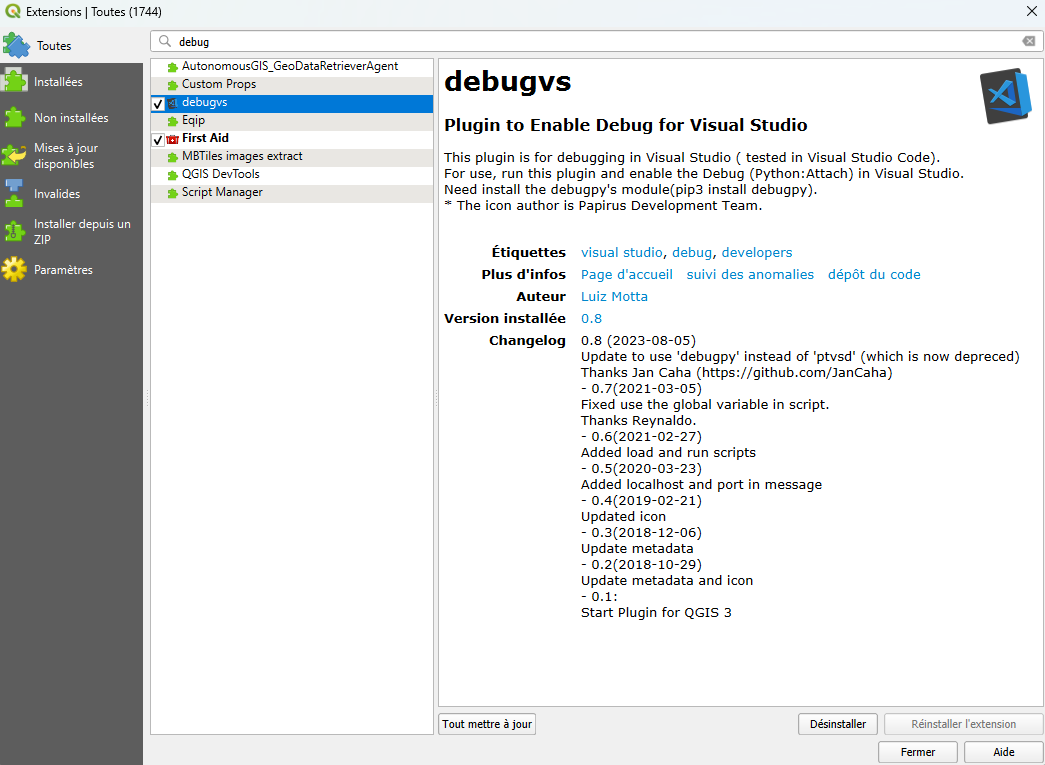
\includegraphics[width=0.6\linewidth]{9_developer_tooling/fig/debugvs.png}
        \caption{\script{debugvs} plugin}
        \label{fig_debugvs}
    \end{figure}
    \item configure VS Code to connect to QGIS during a debugging session:
    \begin{enumerate}
        \item in the CaWaQS-Viz development directory, create a \script{.vscode} sub-directory (add this directory to the \script{.gitignore} file);
        \item create a \script{settings.json} file in the \script{.vscode} sub-directory and copy the content from code \ref{code_settings_vscode}. Optionally modify the directory paths to match your QGIS and Python installation and operating system. This one is for Windows.
        \begin{lstlisting}[language=JSON, caption={Workspace configuration file. This file defines the Visual Studio Code workspace configuration for QGIS plugin development. It adapts the VS Code Python environment to that used by QGIS (installed via OSGeo4W).}, label=code_settings_vscode]
        {

            "workbench.colorCustomizations": {
                "titleBar.activeBackground": "#006823",
                "editor.background": "#000000"
            },

            "python.linting.pylintEnabled": true,
            "python.jediEnabled": true,


            "python.pythonPath": "C:/OSGeo4W64/bin/python-qgis.bat",


            "python.linting.pylintArgs": [
                "--extension-pkg-whitelist=PyQt5,qgis,db_manager",
                "--disable=all",
                "--enable=F,E,unreachable,duplicate-key,unnecessary-semicolon,global-variable-not-assigned,unused-variable,binary-op-exception,bad-format-string,anomalous-backslash-in-string,bad-open-mode"
            ],


            "terminal.integrated.env.windows": {

                "PATH": "C:\\OSGeo4W\\apps\\qgis\\bin;C:\\OSGeo4W\\apps\\Python312;C:\\OSGeo4W\\apps\\Python312\\Scripts;C:\\OSGeo4W\\apps\\Qt5\\bin;C:\\OSGeo4W\\apps\\Python312\\Scripts;C:\\OSGeo4W\\bin;C:\\Windows\\System32;C:\\Windows;C:\\Windows\\system32\\WBem;C:\\OSGeo4W\\apps\\Python312\\lib\\site-packages\\pywin32_system32;C:\\OSGeo4W\\apps\\Python312\\lib\\site-packages\\numpy\\.libs",

                "PYTHONHOME": "C:\\OSGeo4W\\apps\\Python312",
                "PYTHONPATH": "C:\\OSGeo4W\\apps\\qgis\\python;%PYTHONPATH%",

                "GDAL_DATA": "C:\\OSGeo4W\\share\\gdal",
                "GDAL_DRIVER_PATH": "C:\\OSGeo4W\\bin\\gdalplugins",
                "GDAL_FILENAME_IS_UTF8": "YES",

                "GEOTIFF_CSV": "C:\\OSGeo4W\\share\\epsg_csv",

                "O4W_QT_BINARIES": "C:/OSGeo4W/apps/Qt5/bin",
                "O4W_QT_DOC": "C:/OSGeo4W/apps/Qt5/doc",
                "O4W_QT_HEADERS": "C:/OSGeo4W/apps/Qt5/include",
                "O4W_QT_LIBRARIES": "C:/OSGeo4W/apps/Qt5/lib",
                "O4W_QT_PLUGINS": "C:/OSGeo4W/apps/Qt5/plugins",
                "O4W_QT_PREFIX": "C:/OSGeo4W/apps/Qt5",
                "O4W_QT_TRANSLATIONS": "C:/OSGeo4W/apps/Qt5/translations",
                "QT_PLUGIN_PATH": "C:\\OSGeo4W\\apps\\qgis\\qtplugins;C:\\OSGeo4W\\apps\\Qt5\\plugins",

                "QGIS_PREFIX_PATH": "C:/OSGeo4W/apps/qgis",

                "VSI_CACHE": "TRUE",
                "VSI_CACHE_SIZE": "1000000"
            },
            "python.languageServer": "Jedi",
        }
\end{lstlisting}
        \item create a \script{launch.json} file in the \script{.vscode} sub-directory, copy the content from code \ref{code_launch_vscode}, modify the \script{localRoot} and \script{remoteRoot} paths to match your workspace configuration.

        \begin{lstlisting}[language=JSON, caption={VS-Code debugger configuration file. In this configuration, the "connect" section indicates the address and port on which QGIS exposes the debugging session (here localhost:5678). The "pathMappings" block establishes the correspondence between the local project paths open in VS Code (localRoot) and the paths used by QGIS to execute the plugin (remoteRoot). This correspondence is essential for breakpoints placed in VS Code to be correctly associated with the files actually executed by QGIS.}, label = code_launch_vscode]
{
    "version": "0.2.0",
    "configurations": [
        {
            "name": "Attach QGIS Debug",
            "type": "python",
            "request": "attach",
            "connect": {
                "host": "localhost",
                "port": 5678
            },
            "pathMappings": [
                {
                    "localRoot": "C:\\Program Files\\$QGIS$\\apps\\qgis-ltr\\python\\plugins\\cawaqsviz",
                    "remoteRoot": "C:\\Users\\$USER$\\AppData\\Roaming\\QGIS\\QGIS3\\profiles\\default\\python\\cawaqsviz"
                }
            ],
            "justMyCode": false
        }
    ]
}


\end{lstlisting}
        \end{enumerate}
    \item Establish the QGIS/VS-Code connection
    \begin{enumerate}
        \item authorise the debugger connection to QGIS via the \script{debugvs} plugin (\cffig \ref{fig_enable_vscode_qgis});
        \begin{figure}[H]
            \centering
            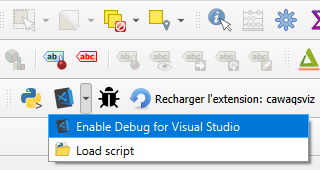
\includegraphics[width=0.40\linewidth]{9_developer_tooling/fig/launch_debug_vs.png}
            \caption{Establishing a QGIS/VS-Code connection from the \script{debugvs} plugin}
            \label{fig_enable_vscode_qgis}
        \end{figure}
        \item launch the VS-Code debugging session (\cffig \ref{fig_debug_VS_CODE}).
        \begin{figure}[H]
            \centering
            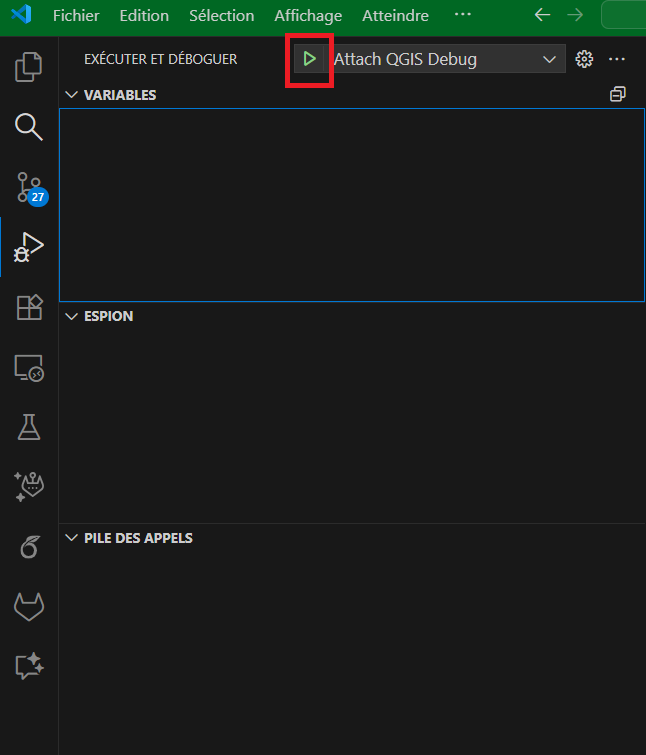
\includegraphics[width=0.5\linewidth]{9_developer_tooling/fig/debug_vs_code.png}
            \caption{Launching a debugging session from VS-Code}
            \label{fig_debug_VS_CODE}
        \end{figure}
    \end{enumerate}
\end{enumerate}

The connection between the debugger and QGIS is terminated from VS-Code by clicking on \script{"Disconnected"} in the debugging toolbar (\cffig \ref{fig_barre_outil_debbug})

\begin{figure}[H]
    \centering
    
\includegraphics[width=0.35\linewidth]{9_developer_tooling/fig/disconnect-debugger.png}
    \caption{VS-Code debugger toolbar}
    \label{fig_barre_outil_debbug}
\end{figure}




\newpage
\section{Creating Dialog Boxes with \script{Qt Designer}}
\label{sec_QtDesigner}
The \script{Qt Designer} application, provided with the QGIS installation (installation with OSGEO), is a tool for creating dialog boxes in the form of .ui files. In the \cwv~application, all dialog boxes have their own \script{.py} file to which the \script{.ui} file, of the same name, is associated with the dialog box's Python class.

\begin{lstlisting}[language = Python, label = code_init_from_ui, caption = Initialisation of the "Compare SIM/OBS" dialog box from a .ui file]
# This loads your .ui file so that PyQt can populate your plugin with the elements from Qt Designer
FORM_CLASS, _ = uic.loadUiType(
    os.path.join(os.path.dirname(__file__), "DialogComparesimobs.ui")
)


class DialogComparesimobs(Dialog, FORM_CLASS):
    def __init__(self, iface:QgisInterface, log_file_path:str, parent=None):
        """Constructor Method

        :param iface: Qgis Interface
        :type iface: QgisInterface
        :param logFilePath: Path of the cawaqs-viz log file, defaults to None
        :type logFilePath: str, optional
        :param parent: Parent class, defaults to None
        :type parent: _type_, optional
        """
        super(DialogComparesimobs, self).__init__(parent)
        self.setupUi(self)
        self.iface = iface
        self.logFilePath = log_file_path
        self.simData = False
\end{lstlisting}
